\section{Beispiele}
	\subsubsection{Mathezeichen fett}
		\begin{equation*}		%Mathe-Umgebung, Gleichung unnummeriert
			\mathbf{B}=B(r) \hat{\phi}=\left\{\begin{array}{ll}{\frac{\mu_{0} I r}{2 \pi a^{2}}} & {r<a} \\ {\frac{\mu_{0} I}{2 \pi r}} & {r \geq a}\end{array}\right.
		\end{equation*}

	\subsection{cases}
		\subsubsection{kompakt}
			$\sum\limits_{n=0}^{\infty}a_n x^n$ Es sei $\lim\limits_{n\to\infty}\sqrt[n]{|a_n|}=\beta \Rightarrow
			\begin{cases}
			\beta=0 & \text{absolut Konvergent für alle } x\in\mathbb{R}\\
			\beta>0 & für 
			\begin{cases}
			\beta=0: & \text { absolut konvergent für alle } x \in \mathbb{R}\\
			|x|>\frac{1}{\beta}: & \text { divergent }\\
			|x|=\frac{1}{\beta} : & \text { keine Aussage möglich }
			\end{cases}\\
			\beta=\pm \infty : & \text { divergent ausser für } x=0
			\end{cases}$\\
		\subsubsection{als aligned}
			$
			D = \left(\frac{a_{1}}{2}\right)^{2}-a_{0} =
			\left\{
			\begin{aligned}
			D>0: & \qquad \lambda_{1,2}=-\frac{a_{1}}{2} \pm \sqrt{\left(\frac{a_{1}}{2}\right)^{2}-a_{0}} & \qquad \in \mathbb{R} & \qquad \text{ starke D"ampfung }
			\\
			D=0: & \qquad \lambda \quad=\quad-\frac{a_{1}}{2} & \qquad \in \mathbb{R} & \qquad \text{ aperiodischer Grenzfall }
			\\
			D<0: & \qquad \lambda_{1,2}=-\frac{a_{1}}{2} \pm j \sqrt{a_{0}-\left(\frac{a_{1}}{2}\right)^{2}} & \qquad \in \mathbb{C}  \backslash \mathbb{R} & \qquad  \text{ schwache Dämpfung / Schwingfall }
			\end{aligned} \right.
			$
			
		\subsubsection{Links rechts Klammer}
			$
			\text{wenn}
			\left.
			\begin{cases}
			{-f(x) \text { auf dem Intervall }[1, \infty) \text { definiert }} \\ 
			{(\text { bzw. }[k, \infty))} \\ 
			{-f(x) \geq 0}\\
			{-f(x) \text { monoton fallend }}
			\end{cases}\right\}
			\Rightarrow
			\begin{cases}{\int\limits_{1}^{\infty} f(x) d x \text { konvergent } \Leftrightarrow \text { Reihe konvergent }} \\ {\int_{1}^{\infty} f(x) d x \text { divergent } \Leftrightarrow \text { Reihe divergent }}\end{cases}
			$\\	
		
		\subsubsection{schöne Darstellung}
			\begin{math}			%Mathe-Umgebung
				\begin{cases}
				{T} & {m=n=1} \\[1.0em]
				{\dfrac{T}{2}} & {m=n>0} \\[1.0em]		%zusätzlicher Abstand und \dfrac oder \frac
				{0} & {m \neq n}
				\end{cases}
			\end{math}
	
	\subsection{Formeln nach Zeichen ausrichten, zB: =}
		$\begin{aligned}[t]
			y^{\prime} &=f\left(\frac{y}{x}\right) \quad
			&|& \text { Substitution: } \quad z=\frac{y}{x} \quad \Leftrightarrow \quad y=z \cdot x \quad(x \neq 0)\\ 
			y^{\prime} &=f(z) \quad &|& 
			\text { differenzieren: } \quad y^{\prime}=z+z^{\prime} \cdot x\\ 
			y^{\prime} &=z+z^{\prime} \cdot x \quad &|& \ y^{\prime}=f(z)\\ 
			f(z) &=z+z^{\prime} \cdot x \quad &|& \ \text{umformen}\\
			z^{\prime}&=(f(z)-z) \cdot \frac{1}{x} &\Rightarrow& \text { separiert! } \quad \text { Anfangsbedingungen: } \quad z_{o}=\frac{y_{0}}{x_{0}}\\
		\end{aligned}$\\
		
	\subsection{compactenum}
		Im Gegensatz zu enumerate und itemize (siehe: Latex-Einführung) ist der Abstand kleiner und perfekt für platzsparende Zusammenfassungen.\\
		$\rightarrow$ usepackage: paralist
		
			\subsubsection{Aufzählung}
					\begin{compactenum}
						\item Homogene DGL lösen: $g(x)=0$ setzen $\rightarrow$ ergibt $Y_H$
						\item Anfangsbedingungen in Hom. DGL einsetzen. Wenn möglich: $x_0=0\quad \newline 
						y_H(x_0)=0 \newline  y_H'(x_0)=1 \qquad$
						\item A, B bestimmen
						\item  Einsetzen der Hom. Glg. in Faltungsintegral 
						$\Rightarrow\quad y_P(x)=\int_{x_o}^{x} y_H(x+x_0-t)\cdot g(t)dt$
						\item $Y=y_H+y_P$
					\end{compactenum}
			
			\subsubsection{Liste}
				\textit{{\color{red}TODO}}		%TODO
				
	%\subsection{Bilder}
	
	\subsection{minipages}
		minipages sind in kurzen Formelsammlungen zu bevorzugen. Aufgrund der möglichen Befehlen und der Platzierung.\\
		\textbf{Minipages dürfen \underline{keine} Abstände zwischen sich haben!!!}\\[1cm]		%Abstand nach Absatz
		
		\subsection{ohne Linien}
			\begin{minipage}{4.5cm}
				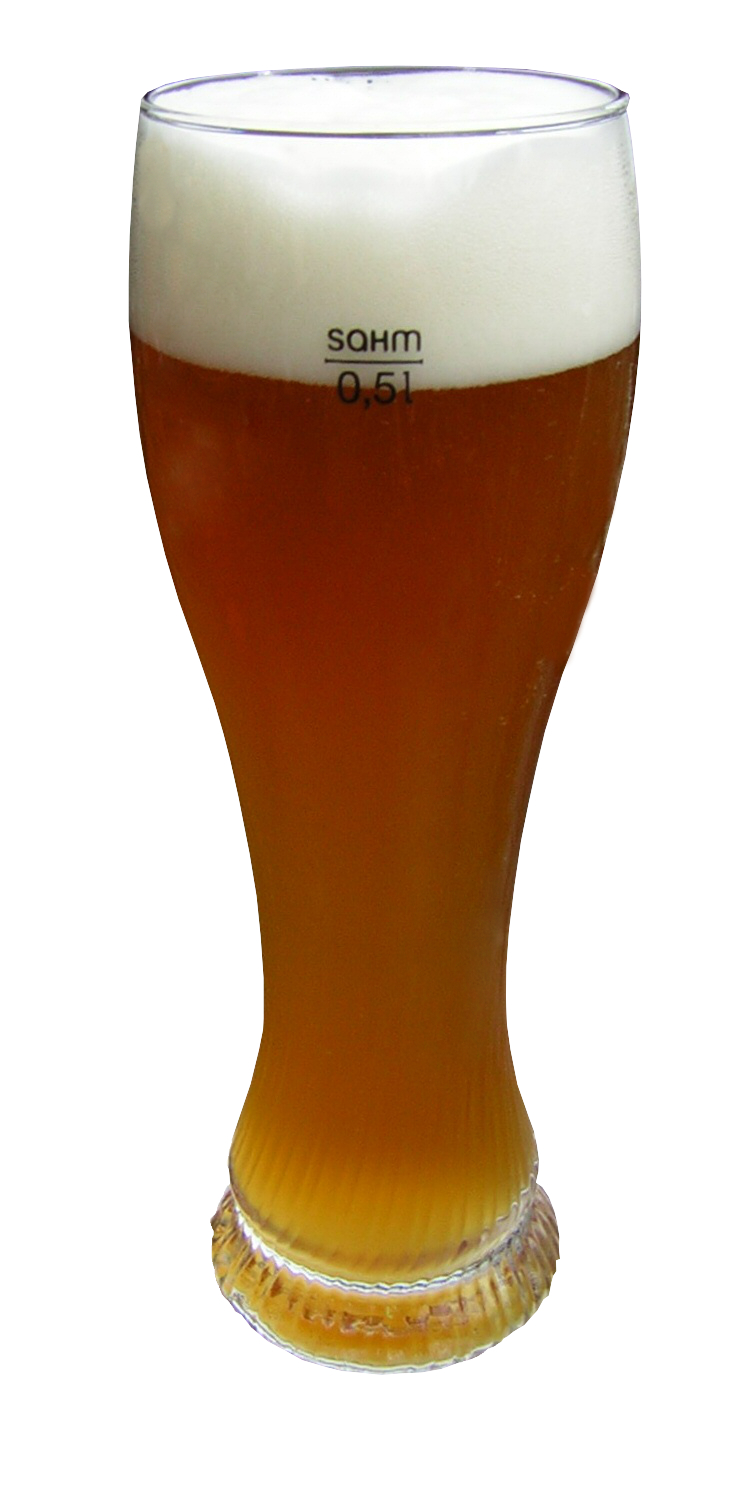
\includegraphics[width=\textwidth]{./images/Weizenbier.jpg}
			\end{minipage} \qquad\qquad				
			\begin{minipage}{0.5\textwidth}
				$\boxed{A^{t} A \vec{x}=A^{t} \vec{b} \quad \Rightarrow \quad \vec{x}=\left(A^{t} A\right)^{-1} A^{t} \vec{b}}$
			\end{minipage}
	
		\subsection{\textbf{mit} Linien}
			\begin{minipage}{4.5cm}
				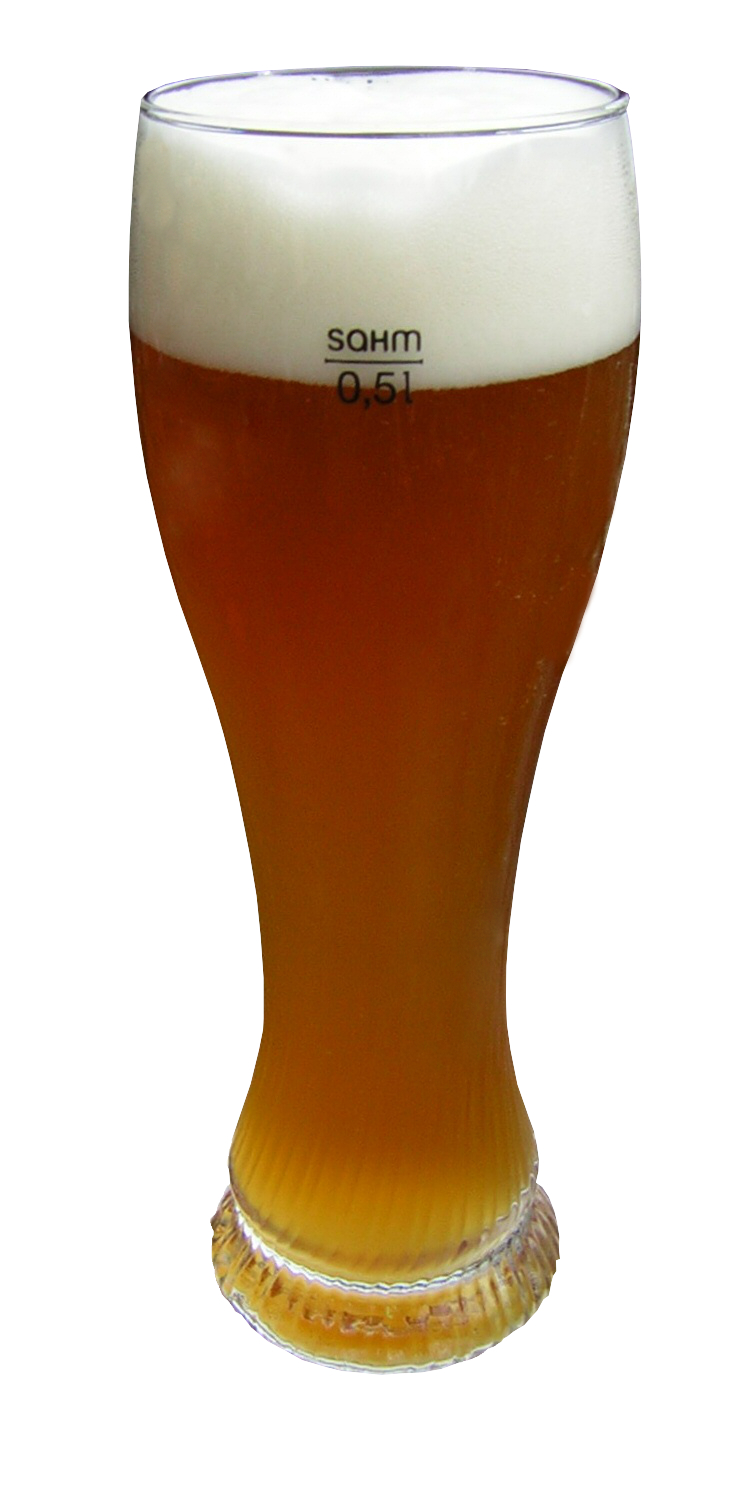
\includegraphics[width=\textwidth]{./images/Weizenbier.jpg}
			\end{minipage} \qquad \vline \qquad			
			\begin{minipage}{0.5\textwidth}
				$\boxed{A^{t} A \vec{x}=A^{t} \vec{b} \quad \Rightarrow \quad \vec{x}=\left(A^{t} A\right)^{-1} A^{t} \vec{b}}$
			\end{minipage}
	
	\subsection{Tabellen}
		benutze: \href{https://tablesgenerator.com}{Tablesgenerator}\\
		\textit{oder}\\
		den Tabellen-Assistenten von TexStudio\\
		
		
	\subsection{weitere Mathebefehle} 
		benutze: \href{https://mathpix.com}{Mathpix}
		
	\subsection{PDF einbinden}
		\subsubsection{Anhang}
			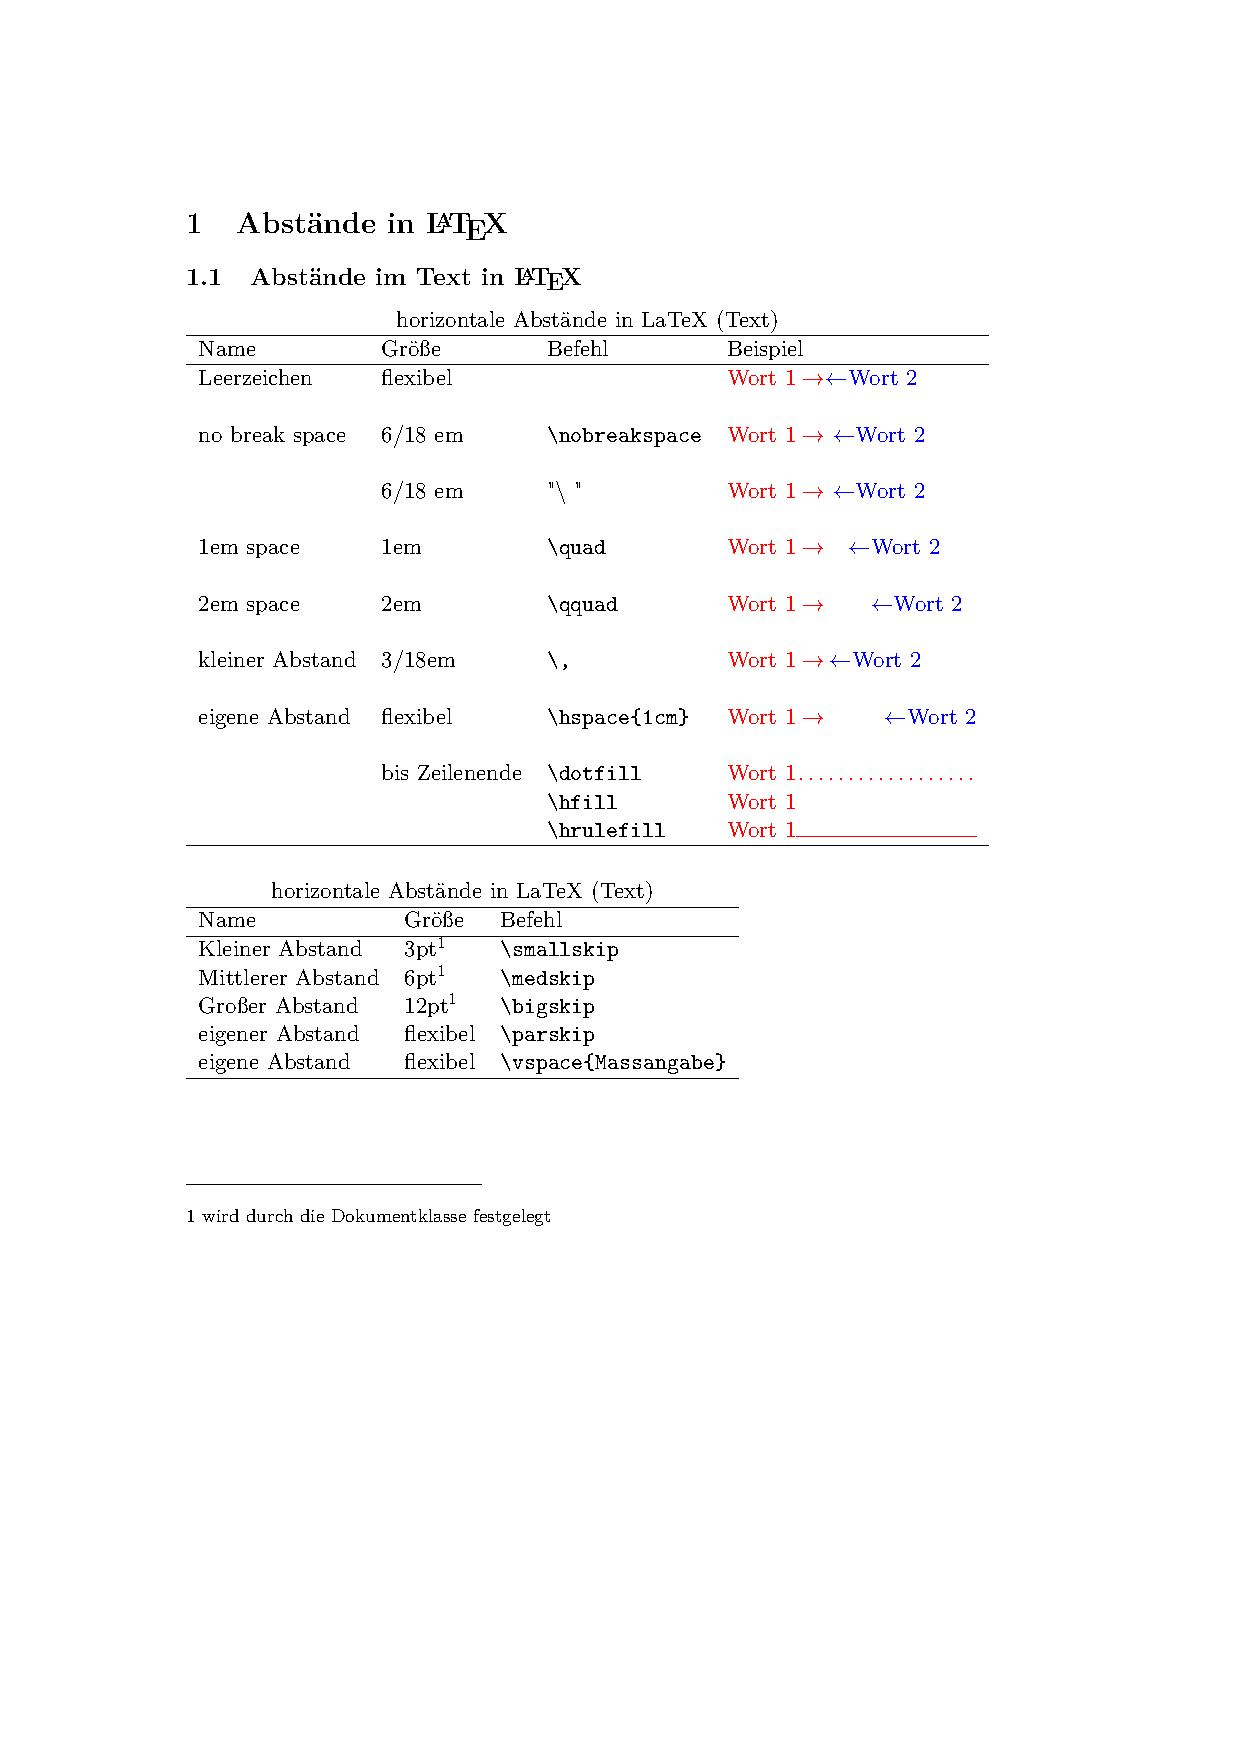
\includepdf[pages=-, scale=1, frame=true]{attachment/AbstaendeInLatex.pdf}		
	
	